\chapter{Scanner}
\label{scanner}
\thispagestyle{empty}

\section{Motivation}
\label{scanner_motivation}
\paragraph{}

CERN Computer Security Team performs scans of various types of resources, such as devices, web servers, web sites, etc. It is impossible to scan these resources manually and there is a need for an Scanning Engine that would facilitate scheduling and running these scans, share the load across multiple scanning hosts in a fault-tolerant way, and combine results.
``GNU Parallel" is a command-line utility for Unix-like operating systems that allows us to execute jobs concurrently locally or using remote computers. A job is typically a single command or a small script that has to be run for each of the lines in the input.\footnote{\url{http://savannah.gnu.org/projects/parallel}} It will be a trivial task to provide GNU Parallel with a list of CERN resources and have the scans run on these resources concurrently.
\\ 
On the other hand, As discussed in section \ref{sec:tools}, CERN has a collection of various scripts for detecting misconfigurations, such as expired certificates and basic HTTP authentication, or vulnerabilities, such as Heartbleed\footnote{Critical OpenSSL security bug disclosed in 2014}. 
\\
There is a need for a tool that fills the gap between detection scripts and GNU Parallel, making it possible to enable the permanent and automatic scanning of the resources. This tool (the Scanner) will act like a wrapper around detection scripts, standardizing the input and output format of the scripts, so that they can be used with GNU Parallel and their results can be analyzed automatically. The Scanner should also make it possible to run a subset of available detection scripts on targets. Another objective of the Scanner is to make it as simple and quick as possible to add a new detection script, and run it on all CERN resources to ensure an acceptable detection/response speed when new vulnerabilities emerge.

\subsection{Use Cases}
\paragraph{}
There are two major use cases for the Scanner:
\begin{itemize}
\item \textbf{Manual execution}: When we need to run an existing set of detection scripts on a new target (or existing targets, to get fresh results), or when we need to create a new script (e.g. Heartbleed test, when OpenSSL vulnerability surfaced) on the usual targets
\item \textbf{Automatic execution}: For permanent scanning of some target lists (e.g. all official web sites, all web servers exposed on the firewall, etc.) with relevant test sets
\end{itemize}

\section{Scanner Specifications}
\paragraph{}
The Scanner runs a set of security tests (called plugins) on a single resource, and collects, combines and outputs plugins scan results. When calling the Scanner, we ask it to scan a given resource type with a unique name. The Scanner ensures only plugins for that resource type will be executed. 

\subsection{Plugin Specifications}
\paragraph{}
A plugin is a single security test for a given type of resource. After scanning a target, it says if a security problem was found or not (It can output more details when relevant). 
%delam gerefte ey doost, havaye gerye ba man...havaye gerye ba man...
\subsubsection{Resource Types}
\paragraph{}
There are various types of resources at CERN. In most cases the plugins need to scan websites or web servers (or other devices), but our implementation of the Scanner is independent of the type of the resource that is being scanned. To avoid complexity, a given plugin should deal with only one type of resource. Occasionally, the same test will need to be developed for different types of resources (e.g default landing page test is needed for both web sites and web server). In that case, the logic of the test should be shared, but still two separate scripts should be developed for each resource type. For example, imagine that the script \texttt{landing\_page.py} contains the logic of testing for a default landing page on websites and web servers. A possible implementation is to develop one script for websites \texttt{landing\_page\_site.sh} that runs `\texttt{./landing\_page.py -site \$1}' and one script for web servers \texttt{landing\_page\_server.sh} that runs `\texttt{./landing\_page.py -server \$1}' 
\subsubsection{Input}
\paragraph{}
The Scanner will provide the plugin with the inputs when running it. Depending on the nature of the security test a plugin is performing, it will need different input data. It is important that all plugins follow a convention about the way they receive the inputs, so that the Scanner can run all the plugins in the same way. The plugin can assume that it is going to receive the input in the following order: \{\texttt{IP/HostName PORT ALIAS URL}\} for web servers/devices and \{\texttt{URL}\} for websites. The plugin can decide to ignore any of these input arguments, if irrelevant. Also, the Scanner might pass an empty string if the user does not specify a field.
\\
Additionally, plugins can be called with the following arguments instead of the target resource:
\texttt{-{}-info} - returns plugin details in JSON format (see Figure \ref{figure:plugin-info})  
\begin{figure}[h!]

  \centering
    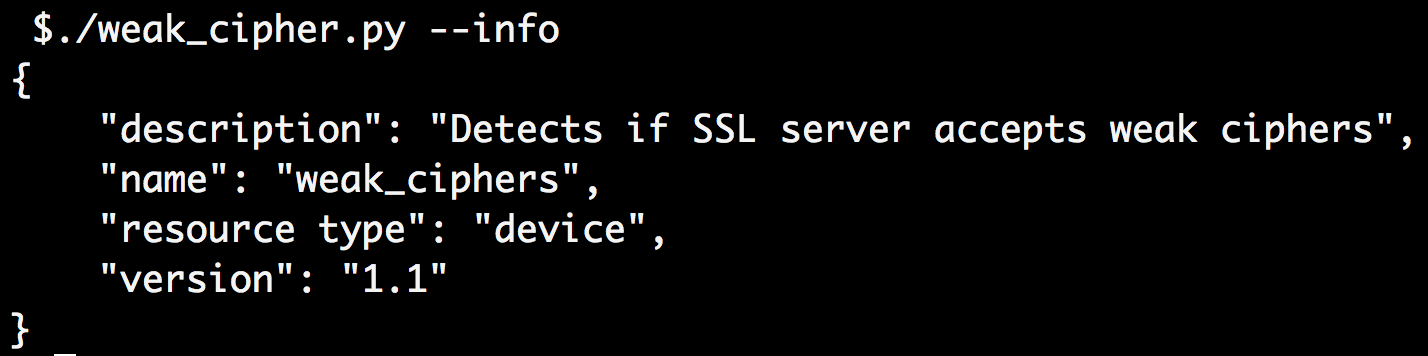
\includegraphics[width=1.0\textwidth]{plugin-info}
  \caption{Plugin Information}
\label{figure:plugin-info}
  
\end{figure}
\subsubsection{Output}
\paragraph{}
It is important that the plugins follow a convention in their output format, so that the Scanner can analyze the results and group them, if necessary. Figure \ref{figure:plugin-results} illustrates a sample plugin output. After scanning a given target, each plugin should return the following information in JSON format (mandatory fields in bold): 
\begin{itemize}


   \item \textbf{result} (mandatory)- severity of the findings; one of these values (Any other value in the result will be accepted by the Scanner, but a warning will be logged.):
    \begin{itemize}
    

        \item \textit{SECURE} - there is no security problem
        \item  \textit{VULNERABLE} - security problem detected
        \item  \textit{WARNING} - there is something sub-optimal (e.g. a certificate expiring soon) but not a real security problem, yet
        \item  \textit{UNKNOWN} - results not available, test couldn't conclude (e.g. host unreachable)
        \item  \textit{TIMEOUT} - results not available, test timed out. (The plugins do not have to detect timeouts as this can be done in the Scanner level) 
            \end{itemize}
\item      \textbf{notes} (mandatory) - human-readable details of the scan result (e.g. which weak ciphers were detected, which URLs are affected)
\item      target (recommended) - what was scanned: If the target information is provided by plugin it will be used to show more precise results, for example if a default port has been used, etc. The plugin can choose to report all or a subset of following:
\begin{itemize}


\item        host
\item    port
\item    alias
\item    url 
\end{itemize}
\item    plugin info (recommended):
\begin{itemize}
\item        name
\item        version
\item    resource type
\item    description - a one-line description of the plugin 
\end{itemize}
\end{itemize}



\begin{figure}[h!]
  \centering
    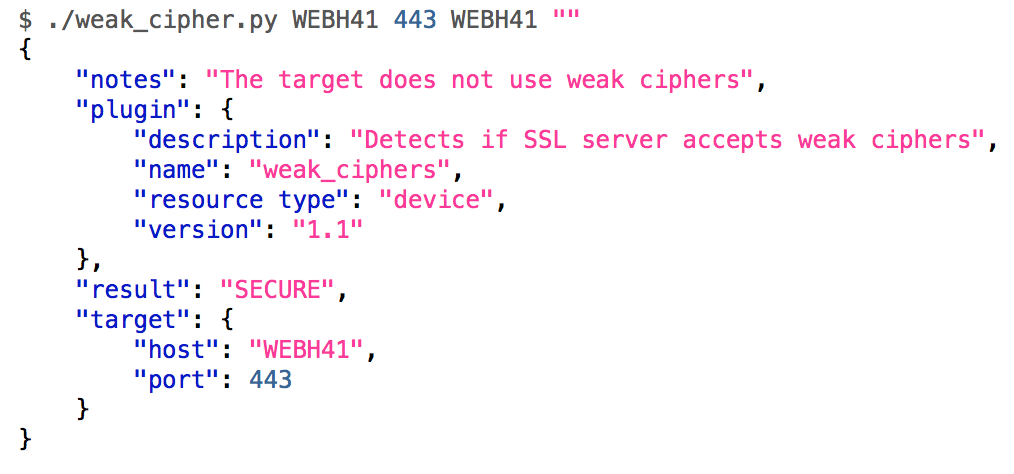
\includegraphics[width=1.0\textwidth]{plugin-results}
  \caption{Plugin Output}
  \label{figure:plugin-results}
  
\end{figure}



\subsection{Scanner Options}
\paragraph{}
The Scanner will be directly used by security team members; therefore, it is important to design a robust user interface for it. The user can use the following options to customize Scanner parameters:

\begin{itemize}

\item 

    \texttt{-l|-{}-list TYPE} - list all plugins available in the plugin directory 
                       (for the given resource type(or all))
\item                  
    \texttt{-n|-{}-no-action} - don't scan    			     (list what will be scanned with which plugins)
\item    \texttt{-q|-{}-quiet} - be quiet
\item    \texttt{    -v|-{}-verbose LEVEL} - be more verbose 
    	 				 (to the given verbosity level in the range of 1 to 5,
    	 				  with 5 being the most verbose)
\item    \texttt{    -t|-{}-timeout SECONDS} - set timeout per plugin (same for all plugins)
\item    \texttt{    --plugin PLUGIN1.sh,PLUGIN2.py,PLUGIN3} - run selected plugins
\item    \texttt{ -{}-plugin-list PLUGINS-FILE} - run plugins listed in the file (one line per plugin executable)
\item    \texttt{  -{}-plugin-dir DIRECTORY} - look for plugins in this directory (default: /opt/scan/plugins)
\item    \texttt{    -{}-log FILE} - log output (but not results) to a file instead on printing on standard output  

\end{itemize}
And the following options can be used to define the target resource:
\begin{itemize}

    \item    \texttt{-{}-device NAME} - scan the device (mandatory for devices)
    \item    \texttt{-{}-website NAME} - scan the centrally hosted website (mandatory for websites)
%    \item    \texttt{-{}-account NAME} - scan the account (mandatory for accounts)
%    \item    \texttt{-{}-set NAME} - scan the set (mandatory for sets)
    \item    \texttt{-{}-ip IPs} - set device target IP addresses (comma separated values)
    \item    \texttt{-{}-port PORTs} - set device target port numbers (comma separated values)
    \item    \texttt{-{}-alias ALIASes} - set device target aliases (comma separated values)
    \item    \texttt{-{}-url URLs} - set device/website target URLs (comma separated values). For devices a url means more like a directory on the device 
   \end{itemize}
   


\subsection{Targets}
\paragraph{}
A CERN resource can be composed of multiple targets. For example, a device can have multiple IP addresses, aliases, open ports or URLs and each combination of these fields can specify a scanning target. A plugin deals with only one target (a single IP, alias, port, etc.) and it is the job of the Scanner to loop over all combinations of IP addresses, aliases, ports and URLs when calling plugins .
\subsubsection{Example}
\paragraph{}
Consider the following command:

\begin{table}[H]
\begin{center}
    \begin{tabular}{ c  l }


\$ \texttt{./scanner.py} &  \texttt{-{}-plugin basic\_auth.py}  \\
			   &  \texttt{-{}-device PCITDI86}  \\
			   &  \texttt{-{}-ip 137.138.43.51,2001:1458::112:33} \\
	           &  \texttt{-{}-port 80,443  }\\
	           &   \texttt{-{}-alias CSC,PHOTOCLUB}  \\
    	       &  \texttt{-{}-url /admin,/tmp}
    	       
	\end{tabular}
    
   \end{center}
\end{table}
\noindent
With this command the Scanner will run the Basic Authentication plugin (which checks if the target is doing the authentication over HTTP instead of HTTPS) on a resource of type `device' and with the name `PCITDI86'. In addition, there are multiple IP addresses, aliases, ports and URLs that we would like to scan. The Scanner is going to run the plugin 2*3*2*2=24 times on PCITDI86. Table \ref{table:targets} shows the different targets that will be scanned. 

\begin{table}
\begin{center}
    \begin{tabular}{ | c | c | c | c |}
    
    \hline
	  \hhline{|*4-}
  \multicolumn{1}{|c|}{\cellcolor{LightBlue}\textbf{IP/Hostname}} & \multicolumn{1}{|c|}{\cellcolor{LightBlue}\textbf{Port}} 
  & \multicolumn{1}{|c|}{\cellcolor{LightBlue}\textbf{Alias}} &    \multicolumn{1}{|c|}{\cellcolor{LightBlue}\textbf{URL}}    
    \\ \hline

   \multirow{12}{*}{137.138.43.51} &     \multirow{6}{*}{80} &     \multirow{2}{*}{PCITDI86} & /admin
   \\
    \cline{4-4}
       &     &     & /tmp
    \\
     \cline{3-4}
	& & \multirow{2}{*}{CSC} & /admin
	\\
	 \cline{4-4}
       &     &     & /tmp
    \\
     \cline{3-4}
 	& & \multirow{2}{*}{PHOTOCLUB} & /admin
	\\
	 \cline{4-4}
       &     &     & /tmp
    \\
     \cline{2-4}
    
    & \multirow{6}{*}{443} &     \multirow{2}{*}{PCITDI86} & /admin
   \\
    \cline{4-4}
       &     &     & /tmp
    \\
     \cline{3-4}
	& & \multirow{2}{*}{CSC} & /admin
	\\
	 \cline{4-4}
       &     &     & /tmp
    \\
     \cline{3-4}
 	& & \multirow{2}{*}{PHOTOCLUB} & /admin
	\\
	 \cline{4-4}
       &     &     & /tmp
    \\
     \cline{1-4}
     
     
     
     
     
     \multirow{12}{*}{2001:1458::112:33} &     \multirow{6}{*}{80} &     \multirow{2}{*}{PCITDI86} & /admin
   \\
    \cline{4-4}
       &     &     & /tmp
    \\
     \cline{3-4}
	& & \multirow{2}{*}{CSC} & /admin
	\\
	 \cline{4-4}
       &     &     & /tmp
    \\
     \cline{3-4}
 	& & \multirow{2}{*}{PHOTOCLUB} & /admin
	\\
	 \cline{4-4}
       &     &     & /tmp
    \\
     \cline{2-4}
    
    & \multirow{6}{*}{443} &     \multirow{2}{*}{PCITDI86} & /admin
   \\
    \cline{4-4}
       &     &     & /tmp
    \\
     \cline{3-4}
	& & \multirow{2}{*}{CSC} & /admin
	\\
	 \cline{4-4}
       &     &     & /tmp
    \\
     \cline{3-4}
 	& & \multirow{2}{*}{PHOTOCLUB} & /admin
	\\
	 \cline{4-4}
       &     &     & /tmp

	
        \\ \hline
    \end{tabular}
    \caption{Targets}
    \label{table:targets}
   \end{center}
\end{table}

For many plugins (e.g. Heartbleed) the URLs are irrelevant, while for others (e.g. basic\_authentication) the possibility to scan several URLs/sub-directories for a given host name is very useful. Obviously, we want to avoid that the Scanner loops over multiple URLs when scanning for Heartbleed. This means that some plugins (e.g. Heartbleed and basic-authentication) should not be used together for the same target details, but rather separately: 

\begin{table}[H]
    \begin{tabular}{ c  l }


\$ \texttt{./scanner.py} & \texttt{-{}-plugin-list https-plugins.txt} \\
  & \texttt{-{}-device PCITDI86} \\
  & \texttt{-{}-alias CSC,PHOTOCLUB}\\
  & \texttt{-{}-port 443,8123}\\
  \\
  
    	       \$ \texttt{./scanner.py} & \texttt{-{}-plugin basic-auth.py} \\
  & \texttt{-{}-device PCITDI86} \\
  & \texttt{-{}-alias CSC,PHOTOCLUB}\\
  & \texttt{-{}-port 80,443,8123}\\
    	       & \texttt{-{}-url /admin,/tmp}
    	       
	\end{tabular}
    
\end{table}
\noindent
If, incidentally or pressed by an emergency, we call the Scanner and provide ``too many" details for plugins which don't need them, things should still work. We just risk waiting for the results a bit longer, and getting duplicated results.
\subsection{Output}
\paragraph{}
The Scanner prints exactly one line per target and vulnerability, semicolon-separated values:
\begin{verbatim}
resource_type;resource_name;plugin_name;result;notes;targets
\end{verbatim}
Targets from the same resource with the same scanning results (results and notes) will be grouped into one line. This gives the plugin designer the opportunity to decide on grouping. For example, if the plugin designer includes the port number in the notes, the targets with the same results but different port numbers will be reported in two different lines. This is useful, because the grouping very much depends on the nature of the test the plugin is running. For example, in the case of Heartbleed, the plugin designer would prefer to include the IP address and port number in the notes, but ignore the URLs. On the other hand, landing\_page plugin would report the complete target fields, including URLs, in the notes.
\subsubsection{Examples}
The following command checks if the device uses SSL3\footnote{SSL version 3 is vulnerable to the POODLE vulnerability discovered in October 2014}:
\begin{table}[H]

    \begin{tabular}{ c  l }


\$ \texttt{./scanner.py} & \texttt{-{}-plugin detect\_ssl3.py } \\
  & \texttt{-{}-device lcg-argus} \\
  & \texttt{-{}-port 443,8443}    	       
	\end{tabular}    

\end{table}
\noindent
The output of the scan is: 
\\
\\
\texttt{
\#resource\_type;resource\_name;test\_name;result;notes;target}
\\
\\
\texttt{device;lcg-argus;detect\_ssl3;VULNERABLE;SSLv3 is enabled on lcg-argus:443;[lcg-argus:443]}
\\
\\
\texttt{device;lcg-argus;detect\_ssl3;VULNERABLE;SSLv3 is enabled on lcg-argus:8443;[lcg-argus:8443]}
\\
\\
As you can see, for each scan a different result line is printed, because the plugin reports the device name and port in the notes. 
This other example checks for a default landing page on a web server:
\begin{table}[H]

    \begin{tabular}{ c  l }


\$ \texttt{./scanner.py} & \texttt{-{}-plugin landing\_page.py } \\
  & \texttt{-{}-device pcitdi86} \\
  & \texttt{-{}-alias pcitdi86-alias}\\    	       
    & \texttt{-{}-url /index.html}\\ 
	\end{tabular}    

\end{table}
\noindent
The output will be:
\\
\\
\texttt{
\#resource\_type;resource\_name;test\_name;result;notes;targets}
\\
\\
\texttt{
device;pcitdi86;landing\_page;SECURE;The target does not use an empty or default page;[pcitdi86-alias(pcitdi86):80/index.html,pcitdi86:80/index.html]
}
\\
In this case, the scanning results of the two targets (with different aliases) are grouped into one line.
If the Scanner faces a problem while running the plugin (plugin crash, output not parsable, etc) it will report a line with the result FAIL. Also, if the user defines a timeout (via -{}-timeout) and a timeout occurs while running the plugin, it will be reported in final results.
\\ 
\texttt{device;pcitdi87;landing\_page;TIMEOUT;plugin timeout after 10 ms;[pcitdi86:80/index.html]}
\\
\\
\texttt{device;pcitdi88;landing\_page;FAIL;There was a problem parsing plugin output(error code 127);[pcitdi86:80/index.html]}
\\
\\
%\section{Implementation}
%\subsection{Directory Structure}
%The plugins directory can be set by using the option -{}-plugin-dir. Each plugin should be placed in its corresponding resource type directory. Therefore, the plugins directory contains the following sub-directories:
%\begin{itemize}
%
%
%   \item \texttt{/device}
%    \item \texttt{/web}
%    \item \texttt{/account}
%    \item \texttt{/site} 
%    
%    \end{itemize}
%
%note that all executable files in these directories are considered plugins. In particular, they all will be executed(!), when we call \texttt{./scanner.py -{}-list TYPE}

\section{Conclusion}
\paragraph{}
The Scanner fills the gap between an Scanning Engine and individual security tests. It makes it easier to develop detection scripts that would test for a misconfiguration or a vulnerability on a single target. This can improve the procedure of scanning CERN resources, whenever a new vulnerability is discovered. Using the Scanner we can develop short detection scripts that deal with only one target and use the Scanner to take care of looping over different targets on the same resource. In one level higher, we would like to scan multiple resources at CERN (maybe the whole CERN infrastructure) to find vulnerable resources, in a concurrent and fault tolerant manner. GNU Parallel as described in section \ref{scanner_motivation} can feed the resource data (from prepared files, obtained by running \texttt{was list-servers} and \texttt{was list-sites}) to the Scanner and have it scan multiple resources concurrently.
\\
In addition, the Scanner will group the findings of individual tests to remove duplicate results and generate a parsable output that can be used for further investigations. For example. the Scanner output can be inserted into CERN System Security DataBase (SSDB), used to keep track of vulnerabilities. Integration to SSDB is not implemented, yet, because the team is planning to replace SSDB with an alternative solution. 

